\begin{activity} \label{A:5.6.3}  Consider the functions $f(x) = 2-x^2$, $g(x) = 2-x^3$, and $h(x) = 2-x^4$, all on the interval $[0,1]$.  For each of the questions that require a numerical answer in what follows, write your answer exactly in fraction form.
\ba
	\item On the three sets of axes provided in Figure~\ref{F:5.6.Act3}, sketch a graph of each function on the interval $[0,1]$, and compute $L_1$ and $R_1$ for each.  What do you observe?
	\item Compute $M_1$ for each function to approximate $\int_0^1 f(x) \,dx$, $\int_0^1 g(x) \,dx$, and $\int_0^1 h(x) \,dx$, respectively.
	\item Compute $T_1$ for each of the three functions, and hence compute $S_1$ for each of the three functions.
	\item Evaluate each of the integrals $\int_0^1 f(x) \,dx$, $\int_0^1 g(x) \,dx$, and $\int_0^1 h(x) \,dx$ exactly using the First FTC.
	\item For each of the three functions $f$, $g$, and $h$, compare the results of $L_1$, $R_1$, $M_1$, $T_1$, and $S_1$ to the true value of the corresponding definite integral.  What patterns do you observe?
\ea
\begin{figure}[h]
\begin{center}
\scalebox{0.9}{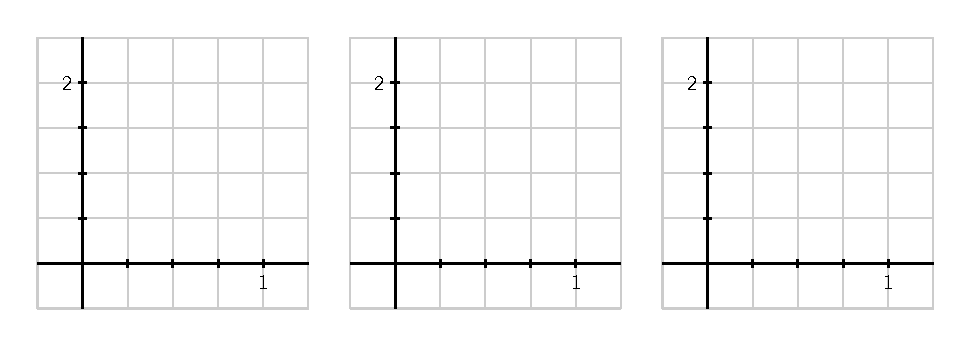
\includegraphics{figures/5_6_Act3.eps}}
\caption{Axes for plotting the functions in Activity~\ref{A:5.6.3}.} 
\label{F:5.6.Act3}
\end{center}
\end{figure}
\end{activity}
\begin{smallhint}
\ba
	\item Small hints for each of the prompts above.
\ea
\end{smallhint}
\begin{bighint}
\ba
	\item Big hints for each of the prompts above.
\ea
\end{bighint}
\begin{activitySolution}
\ba
	\item Solutions for each of the prompts above.
\ea
\end{activitySolution}
\aftera